\section{Applications}
\label{sec:app}

In any scientific discipline, where for studying the object of research, the scientist need to process (large scale) image/video datasets, CV technology can be applied.  For many decades, CV techniques have been applied widely and become standard tool in many scientific applications. Examples are remote sensing (imaging Earth of pa planet), electrical resistivity imaging (geophysical method to image the underground), sonar and radar imaging, and one of the most important applications- (bio)medical imaging. Here, only a few examples of recently emerging application domains are given, even more new challenges will appear when scientists from different domains become aware of the capabilities and potential of the CV technology.

\subsection{Animal biometrics}
\label{sec:anim_biom}
In \cite{Kuehl2013}, Kuehl and Burghardt give overview of the methodologies and trends in the emerging field of {\em animal biometrics}. It is an exciting field operating at the intersection between pattern recognition, ecology and information sciences. The subject of the field is to produce computerized systems for phenotypic measurement and interpretation. The main questions for which such systems helps to find the answers to are: how to profile species, individuals and animal behavior by representing phenotypic appearance. Figure \ref{fig:photoIDpen} illustrates the main components of a biometric system. 

\begin{figure}[H]
\begin{center}
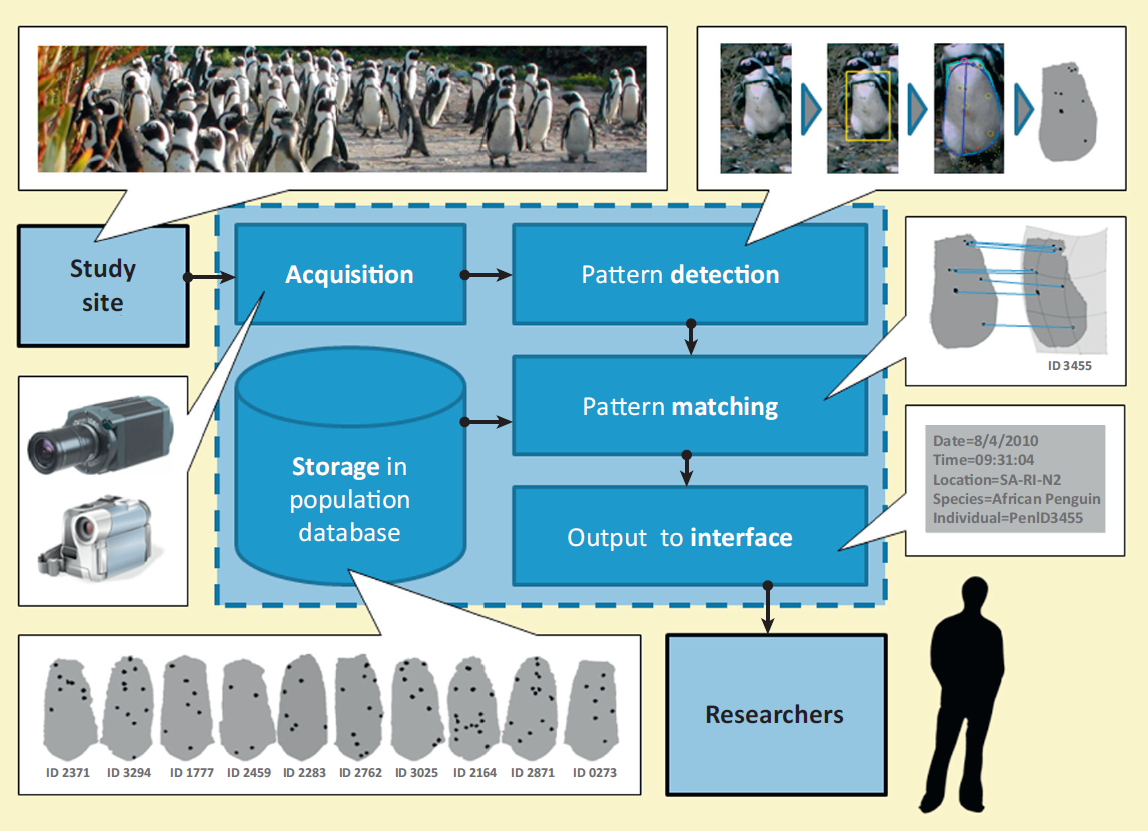
\includegraphics[width=0.68\textwidth]{fig/PhotoIDPenguins}
\end{center}
\caption{Main components of an animal biometric system. This flowchart summarizes how information from a study site is measured and interpreted for the researcher by
an animal biometric system.}
\label{fig:photoIDpen}
\end{figure}
The system parts can either be connected directly on-site or remotely via networks. Each of the components is illustrated, using individual African penguin recognition by spot pattern as an example.  Acquisition: automatic or semi-automatic collection of images or video from fixed field cameras, observers or
the general public. Detection: the use of computer algorithms to search the images to find those that contain the biometric entity of interest and then to extract relevant
information about that entity (e.g., the chest spots of a penguin). Storage: the extracted data on the entity is reduced to a compact mathematical form that can be stored in a
suitable database. Matching: the mathematical data on the entity are then compared with other data already stored in the database to find matches that enable the
individual or the behavior to be identified, using methods akin to the matching of fingerprints to identify humans. Interfacing: presenting the output of the biometric system
to a user or software system for further analysis.

Animal biometrics is important field not only for ecological researchers, but for the general public. For example, in \cite{Kumar2014}, a biometric system for face recognition of pet animals (mainly dogs) have been developed.

\subsection{Plant identification}
Similar field is automatic plant identification. This is an example of the Classification task (What is my object?). Often the identification of trees and flowers is performed from images of the leaves of the plant. Nowadays, many \href{http://www.gardenista.com/posts/diy-identify-leaves-and-flowers-theres-an-app-for-that}{\underline{mobile app}s} exist for the general public.

One such CV system is \href{http://neerajkumar.org/projects/leafsnap/}{\underline{Leafsnap}}, \cite{leafsnap}. Its goal is to assist botanists by automating the tedious and error-prone process of identifying existing plant species. 

The recognition process, developed by the research groups from Columbia University and University of Maryland, consists of, \cite{leafsnap_eccv2012}:
\begin{enumerate}
\item{ {\bf Segmenting} the image to obtain a binary image separating the leaf from the background. This is implemented using an Expectation-Maximization framework, estimating foreground and background color distributions in the HSV color-space.}
\item{{\bf Extracting features} from the binarized image for compactly and discriminatively representing the shape of the leaf. The features used are histograms of curvature over scale as the feature representation, robustly and efficiently implemented using integral measures of curvature.}
\item{{\bf Comparing the features} to those from a labeled database of leaf images and returning the species with the closest matches. Due to the discriminative power of the features and the size of our labeled dataset, we use a simple nearest neighbor approach with the $L_1$-norm.}
\end{enumerate}
The system has the same components as that of an animal biometric system (Figure \ref{fig:photoIDpen}), which indicates, that plan biometrics is a very similar application domain to animal biometrics.

Figure \ref{fig:Leafsnap} gives an impression of the functionality of Leafsnap.

The example of tree species identification (see the \underline{\nameref{sec:intro}} section) is another problem from the same domain. Also, in a the current NLeSC project \href{https://www.esciencecenter.nl/project/prediction-of-candidate-genes-for-traits-using-interoperable-genome-annotat}{\underline{candYgene}} image-based classification of different tomato species collected from different places in the world could be applied. 
\begin{figure}[H]
\begin{center}
\includegraphics[width=0.95\textwidth]{fig/LeafSnap}
\end{center}
\caption{Tour of the iPhone version of Leafsnap.}
\label{fig:Leafsnap}
\end{figure}



\subsection{Computer forensics}
{\em  Forensic Science} is the application of knowledge from several branches of science to answer questions relevant to a legal system. Due to the evolution of criminal activities, more
specialized disciplines have been involved, such as Computer Science, Engineering and Economics.
The research field that unites the fields of Forensic Science and Computer Science is called {\em Computer (Digital) Forensics} and encompasses the study of research methods, driven by
hypothesis, of a specific problem, through the use of computers and computational methods.

Many questions in digital forensics can be answered (or assisted) by CV technologies, such as face detection and identification, same object/scene identification, image/video categorization, camera identification etc. for which the presented earlier CV methods are very highly applicable.

There are also specific problems for example, photogrammetry, 3D  reconstruction  of  impressions, reconstruction of fragmented documents and images etc. Research is done in novel CV methods which help solve these problems, \cite{Andalo13SIBGRAPI}.

\subsection{Social signal processing}
In the last years, a multi-disciplinary area, called {\em Social  Signal  Processing} emerged where computer vision and social sciences converge.  One of the research topics is the development of video surveillance  algorithms to help studying social interactions. Technologically the problems are those of gesture (frequency) analysis, gait, pose and emotion recognition, geometric configuration of people, etc. (Figure \ref{fig:SSP}). A survey of this domain with presentation of the main applications and research results can be found in \cite{Vinciarelli:2009}. 

\begin{figure}[H]
\begin{center}
\includegraphics[width=0.75\textwidth]{fig/SSP}
\end{center}
\caption{Behavioral cues and social signals. Multiple behavioral cues (vocal behavior, posture, mutual gaze, interpersonal distance, etc.) combine to produce a social signal
(in this case aggressivity or disagreement).}
\label{fig:SSP}
\end{figure}


\href{http://www.measuringbehavior.org/}{\underline{\em Measuring behavior }} is the premier interdisciplinary event for scientists and practitioners concerned with the study of human or animal behavior. The biannual conference is held traditionally in the Netherlands. At the same time, the CV community becomes more aware of these applciaiton areas, for example one \href{http://www.seas.upenn.edu/~hypar/GroupBehavior/cvpr15_tutorial_group_behavior.html}{\underline{tutorial}} at the Computer Vision ad Pattern Recognition (CVPR) conference 2015 was on ``Group Behavior Analysis and Its Applications''.